\section{Operads}

\begin{frame}{}
    \tableofcontents[currentsection]
\end{frame}

\begin{frame}{Operads Definition}
      \begin{defin}
        An {\em operad} $\O$ in $\C$
        consists of 
        \begin{itemize}
        \item a family of objects $(\O(j))_{j \in \N}$
        \item a unit morphism $\eta \colon k \rightarrow \O(1)$
        \item a composition morphism
        \[
            \gamma \colon \O(k) \otimes \O(j_1) \otimes \cdots \otimes \O(j_k) \rightarrow \O(j),
        \]
        where $\sum_{1 \leq i \leq k} j_i = j$ 
        \item an action of $S_n$ on $\O(n)$ 
        \end{itemize}
        such that suitable
        associativity, equivariance, unitality constraints hold.
      \end{defin}
\end{frame}

\begin{frame}{Little Disk Operad in $\Top$}
  Let $\dd^2$ be the closed unit disk in $\R^2$. 
  A \emph{little disk} is
  an embedding $f \colon \dd^2 \to \dd^2$ of the following form:
  \[
    f(r_1, r_2) \coloneqq (c_1, c_2) 
  + \lambda(r_1, r_2)
  \]
  for $(c_1, c_2) \in \dd^2$ and $\lambda \in \R$ such that
  \[
      0 < \lambda \leq 1 - \sum_{i=1}^{2} c_i^2.     
  \]
  \[
      \E_2(k) \coloneqq \left\{ f_1 \sqcup \dots \sqcup f_k  \colon \inter(f_i) \cap \inter(f_j) = \emptyset \right\}.
  \]
\end{frame}


\begin{frame}[fragile]{Little Disk Operad in $\Top$}
  Composition map is defined by ``inserting configurations'':
\[
\begin{aligned}
  \gamma \colon \E_2(k) \times \E_2(j_1) \times \dots \times \E_2(j_k) &\to \E_2(j) \\
  (c, c_1, \dots, c_k) &\mapsto c(c_1, \dots, c_k)
  \end{aligned}
\]
  
  \begin{center}
  \begin{adjustbox}{max width=11cm}
      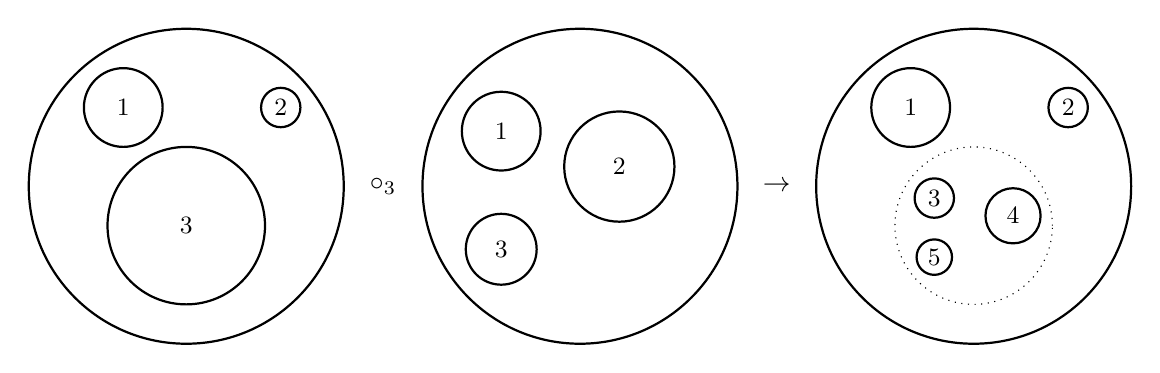
\begin{tikzpicture}
        % First element (left)
        \draw[thick] (-3,0) circle (2); \draw[thick] (-3.8, 1)
        circle (0.5); \draw[thick] (-1.8, 1) circle (0.25);
        \draw[thick] (-3, -0.5) circle (1); \node at (-3.8, 1)
        {\small $1$}; \node at (-1.8, 1) {\small $2$}; \node at (-3,
        -0.5) {\small $3$};
    
        \node at (-0.5,0) {$\circ_3$};

        \draw[thick] (2,0) circle (2); 
        \draw[thick] (1,0.7) circle (0.5); 
        \draw[thick] (2.5,0.25) circle (0.7); 
        \draw[thick] (1,-0.8) circle (0.45); 
        \node at (1,0.7) {\small $1$}; 
        \node at (2.5,0.25) {\small $2$}; 
        \node at (1,-0.8) {\small $3$};
                        
        \node at (4.5,0) {$\rightarrow$};
                  
        \draw[thick] (7,0) circle (2);
        \draw[thick] (6.2, 1) circle (0.5);
        \draw[thick] (8.2, 1) circle (0.25);
        \draw[dotted] (7, -0.5) circle (1);
        \draw[thick] (6.5, -0.15) circle (0.25);
        \draw[thick] (7.5, -0.375) circle (0.35);
        \draw[thick] (6.5, -0.9) circle (0.225);
        \node at (6.2, 1) {\small $1$};
        \node at (8.2, 1) {\small $2$};
        \node at (6.5, -0.15) {\small $3$};
        \node at (7.5, -0.375) {\small $4$};
        \node at (6.5, -0.9) {\small $5$};
      \end{tikzpicture}
  \end{adjustbox}
  \end{center}

\end{frame}

\begin{frame}[fragile]{Cocartesian Morphism}
    \begin{defin}
     Let $P \colon \C \to \D $ be a functor.
        We call a morphism $f_! \colon x \to y$ in $\C$ {\em cocartesian} if for any morphism $g \colon  y \to z$ in $\C$ and
        $\omega \colon P(x) \to P(z)$ in $\D$ with $\omega \circ P(f) = P(g)$,
        there is a unique morphism $\omega' \colon x \to z$ such that
        $P(\omega')=\omega$ and $\omega' \circ f = g$. In a diagram this results
        in the following:
        \begin{center}
         \begin{tikzcd}
                y \arrow[r, "g"] \arrow[rd, "f_!"'] & z                                & {} \arrow[r, "P"] & {} & P(y) \arrow[r, "P(g)"] \arrow[rd, "P(f)"'] & P(z)           \\
                                             & x \arrow[u, "\exists! \omega'"', dotted] &                   &    &                           & P(x) \arrow[u, "\omega"']
            \end{tikzcd}
        \end{center}
      \end{defin}

      \begin{defin}
        We call $P$ a (Grothendieck) op-fibration if for any $X$ in $\C$ and $f \colon P(X) \to Z$ in $\D$, there is a cocartesian lift $f_! \colon X \to Y$ in $\C$, $P(f_!)=f$.
      \end{defin}
\end{frame}

\begin{frame}[fragile]{Colored Operads}
  \small{\begin{defin} 
    A {\em colored operad} $\O$ consists of:
    \begin{enumerate}[(i)]
        \item A collection $\{X,Y,Z, \dots\}$ of
        \emph{colors}.
        \item For colors $\{X_i\}_{i \in I}$,
        color $Y$, a {\em set of morphisms}:
        $\Mul_{\O}(\{X_i\}_{i \in I}, Y)$.
        \item For a finite map $I \to J$ with fibers $I_j$, $j \in J$, 
        % collections of colors $\{X_i\}_{i \in I}$, $\{Y_j\}_{j \in J}$,
        % color $Z$, 
        a composition map:
        \[
            \prod_{j \in J} \Mul_{\O}(\{X_i\}_{i \in I_j}, Y_j) \times \Mul_{\O}(\{Y_j\}_{j\in J}, Z) \to \Mul_{\O}(\{X_i\}_{i \in I}, Z).  
        \]
        \item For every color $X$ an identiy morphism $\id_X \in \Mul_{\O}(\{X\},X)$.
        \end{enumerate}
        The data needs to fulfill suitable associativity and unitality conditions.

  \end{defin}}
\end{frame}

\begin{frame}{Symmetric Monoidal Category As Colored Operad}
  \small{\begin{eg}
 Let $\C$ be a symmetric monoidal category. By setting for a finite
        family of objects $\{X_i\}_{i \in I}$ and object $Y$ in $\C$:
        \[
            \Mul_{\C}(\{X_i\}_{i \in I}, Y) \coloneqq \Hom(\otimes_{i \in I} X_i, Y),
        \]
        % \todo{define order of tensoring: what is our convention? (from left to
        % right)}
        we can define a colored operad $\C$. The composition is given by
        \begin{align*}
            \prod_{j \in J} \Hom(\otimes_{i \in I_j} X_i, Y_j) \times \Hom(\otimes_{j \in J} Y_j, Z) &\to \Hom(\otimes_{i \in I} X_i, Z) \\
            ((f_j)_{j \in J}, g) &\mapsto g \circ (\otimes_{j \in J} f_j) \\
        \end{align*}
        with $\{ \id_X\}_{X \in \C}$ being the unit.
      \end{eg}}
\end{frame}

\begin{frame}{Finite Pointed Sets}
    \begin{defin}
        The {\em category of finite pointed sets} $\Fin$ is defined as
        follows:
        \begin{itemize}
            \item An objects of $\Fin$ is $ 
            \langle n \rangle \coloneqq \{1, \dots, n, \ast\} $ for all $n \in \N$.
            \item A morphism $\alpha \colon \langle n \rangle \to \langle m
            \rangle$ is a map of finite sets where $\alpha(*)=*$.
        \end{itemize}
    \end{defin}
\end{frame}

\begin{frame}{Categorical Definition of $\O$}
   \begin{defin}\label{def:Ox} \small{For $\O$ being a colored operad, the category $\Ox$
    is defined in the following way:
    \begin{enumerate}[(i)]
        \item The objects of $\Ox$ are finite sequences of colors of $\O$.
        \item For $\{X_i\}_{1 \leq i \leq m}$, $\{Y_j\}_{1 \leq j \leq n}$
        objects in $\Ox$. A morphism
            $\phi \colon \{X_i\}_{1 \leq i \leq m} \to \{Y_j\}_{1 \leq j \leq n}$
        is given by
        
        \begin{itemize}
          \item $\alpha \colon \langle m \rangle \to \langle n
        \rangle$ map in $\Fin$.
        \item family of morphisms
        \[
            \{ \phi_j \in \Mul_{\O}(\{X_i\}_{i \in \alpha^{-1}(j)}, Y_j)\}_{1 \leq j \leq n}
        \]
        in $\O$.
        \end{itemize}
        
        \item Composition of morphisms $\phi, \phi'$ is determined by the composition in
        $\Fin$ and $\O$, i.e. $\bar{\alpha} = \alpha'\circ \alpha$ and
        $
            (\phi' \circ \phi)_l \in  \Mul_{\O}(\{X_i\}_{i \in \bar{\alpha}^{-1}(l)}, Z_l)%\}_{1 \leq l \leq k},
        $
        % where $(\phi' \circ \phi)_l$ is applying the following composition map
        % to $((\phi_i)_{i \in \alpha^{-1}(l)}, \phi'_l)$
        by applying $\gamma$ to $((\phi_i)_{i \in \alpha^{-1}(l)}, \phi'_l)$
        % \[
        %     \gamma \colon \prod_{j \in \alpha'^{-1}(l)} \Mul_{\O}(\{X_i\}_{i \in \alpha^{-1}(j)},Y_j) \times \Mul_{\O}(\{Y_i\}_{i \in \alpha'^{-1}(l)},Z_l) \to \Mul_{\O}(\{X_i\}_{i \in \bar{\alpha}^{-1}(l)},Z_l).
        % \]
    \end{enumerate}}
\end{defin}
\end{frame}

\begin{frame}{Categorical Definition of $\O$}
  Let $\O$ be a colored operad. There is a forgetful functor 
\[
\pi \colon \Ox \to \Fin
\]
\pause
  \begin{prop}\label{m1m2} If $\O$ was induced by a symmetric monoidal category $\C$, then:
    \begin{enumerate}[(M1)]
        \item \textbf{Op-fibration condition:} $\pi$ is a Grothendieck
        op-fibration. 
        \item \textbf{Segal condition:} $\C \cong
        \Ox_{\langle 1 \rangle}$ and
        $\Ox_{\langle n \rangle} \cong \C^n$.
    \end{enumerate}
  \end{prop}
\pause
  \begin{prop}
    $$\{\text{symmetric monoidal categories}\} \cong \left\{\begin{aligned}\text{op-fibrations } \D \to \Fin \\
      \text{ satisfying Segal condition}\end{aligned}\right\}$$
  \end{prop}
\end{frame}

% \begin{frame}[fragile]{Symmetric Monoidal Structure on $\mathcal{C} \coloneqq \mathcal{D}_{\langle 1 \rangle}$}
% Let $\pi \colon \mathcal{D} \to \mathrm{Fin}$ a functor satisfying (M1) and (M2).

% \centering
% \renewcommand{\arraystretch}{1.9} % Increase row height for better readability
% \begin{tabular}{|p{0.45\textwidth}|p{0.45\textwidth}|}
% \hline
% $\mathcal{D}$ & $\mathrm{Fin}$ \\
% \hline
% tensor product: \\ $\bigotimes \colon \mathcal{C}^2 \cong \mathcal{D}_{\langle 2 \rangle} \rightarrow \mathcal{C}$ & $\alpha \colon \langle 2 \rangle \to \langle 1 \rangle$ active \\
% \hline
% braiding: $b_{A,B} \colon A \otimes B \cong B \otimes A$ & $\begin{aligned}
% \beta \colon \langle 2 \rangle &\to \langle 2 \rangle \\
% 1 &\mapsto 2 \\
% 2 &\mapsto 1
% \end{aligned}$ \\
% \hline
% associator: $a_{A,B,C} \colon (A \otimes B) \otimes C \cong A \otimes (B \otimes C)$ & $\begin{aligned}
% \tau^3_i \colon \langle 3 \rangle &\to \langle 2 \rangle \\
%  j &\mapsto \begin{cases}
%  j & 1 \leq j \leq i \\
%  j-1 & i < j \leq n \\
% \ast & j=\ast
% \end{cases}
% \end{aligned}$ \\
% \hline
% tensor unit: $\mathcal{D}_{\langle 0 \rangle} \to \mathcal{C}$ & $\eta \colon \langle 0 \rangle \to \langle 1 \rangle$ \\
% \hline
% \end{tabular}
% \end{frame}

\begin{frame}[fragile]{Symmetric Monoidal Structure on $\mathcal{C} \coloneqq \mathcal{D}_{\langle 1 \rangle}$}
Let $\pi \colon \mathcal{D} \to \Fin$ an op-fibration satisfying the Segal condition.

Let $\mu \colon \langle 2 \rangle \to \langle 1 \rangle$ active morphism in $\Fin$.
Then for every $(A,B) \in \C^2$ there is a cocartesian lift $\mu$: $(A,B) \to A \otimes B$.
Thus, a functor
\[
   \bigotimes \colon \mathcal{C}^2 \rightarrow \mathcal{C}
\]
For $\beta \colon  \langle 2 \rangle \to \langle 2 \rangle$ with $\beta(1)=2$, $\beta(2)=1$. We lift the following diagram:
\[
% https://tikzcd.yichuanshen.de/#N4Igdg9gJgpgziAXAbVABwnAlgFyxMJZABgBpiBdUkANwEMAbAVxiRAAoBBUgIQEoQAX1LpMufIRQBGclVqMWbdj1KcBw0djwEiMqXPrNWiEDwAEAHQsQ8AW3hnOQkSAxaJRMvuqHFJzpbWdg48zpriOigAzLI+CsYgVgx0YADmDDBmAEyBAE4p6awarmLaksgALLHyRmxJBRnZeQ1FLm4R5THeNX6JFslpjVLNg63hZURV3b4J9aNmw1b5o0JyMFCp8ESgAGa5ELZIZCA4EEhSxXsHR9SnSDEgyQBGMAwACqUeJrlYqQAWOBAcVqJisNiw9gQl32h0QMhOZ0QWWBvTBwShLiusIedyR1AYWDACSgdDgf3WQJ6CSeYRAWKQVQRSAAbCjZhZbExKc9Xh93JEQD9-oDoddEIzcQBWNl1CwvHB0Wn0xDSpmIADsMtBHK5othrLVmqpsqwUFWgiAA
\begin{tikzcd}
{(A,B)} \arrow[r] \arrow[d, "\otimes"'] & {(B,A)} \arrow[d, "\otimes"] & {\overset{\pi}{\rightarrow}} & \langle 2 \rangle \arrow[d, "\mu"'] \arrow[r, "\beta"] & \langle 2 \rangle \arrow[d, "\mu"] \\
A \otimes B \arrow[r, "b", dashed]      & B \otimes A                  &  & \langle 1 \rangle \arrow[r, "\id"]                     & \langle 1 \rangle                 
\end{tikzcd}
\]

Thus, we have a symmetric braiding:
\[
  b_{A,B} \colon A \otimes B \cong B \otimes A
\]  
\end{frame}

% \begin{frame}{Symmetric Monoidal Structure on $\mathcal{C} \coloneqq \mathcal{D}_{\langle 1 \rangle}$}
% associator: $a_{A,B,C} \colon (A \otimes B) \otimes C \cong A \otimes (B \otimes C)$
  
% $\begin{aligned}
% \tau^3_i \colon \langle 3 \rangle &\to \langle 2 \rangle \\
%  j &\mapsto \begin{cases}
%  j & 1 \leq j \leq i \\
%  j-1 & i < j \leq n \\
% \ast & j=\ast
% \end{cases}
% \end{aligned}$

% tensor unit: 
% $\mathcal{D}_{\langle 0 \rangle} \to \mathcal{C}$ to $\eta \colon \langle 0 \rangle \to \langle 1 \rangle$ 

% \end{frame}


\begin{frame}{$\infty$-operad}
    \small{\begin{defin}
    An $\infty${\em-operad} is a functor $p \colon \Ox \to \nerv(\Fin)$ of
    $\infty$-categories such that:
    \begin{enumerate}[(i)]
        \item For every inert morphism $f \colon \langle n \rangle \to \langle m
        \rangle$ in $\nerv(\Fin)$, object $C \in \Ox_{\langle m \rangle}$,
        there is a $p$-cocartesian morphism $f \colon C \to C'$ in $\Ox$
        lifting $f$. 
        % In particular $f$ induces a functor $f_{!} \colon
        % \Ox_{\langle n \rangle} \to \Ox_{\langle m \rangle}$.
        \item Let $C \in \Ox_{\langle m \rangle}$ and $C' \in \Ox_{\langle n
        \rangle}$ be objects, $f : \langle m \rangle \to \langle n \rangle$ be a
        morphism in $\Fin$ and let $\Map_{\Ox}^f(C, C')$ be the union of
        connected components of $\Map_{\Ox}(C, C')$ which lie over $f$. Choose
        $p$-cocartesian morphisms $C' \to C'_i$ lying over the inert morphism
        $\rho^i \colon \langle n \rangle \to \langle 1 \rangle$ for $1 \leq i
        \leq n$. Then the induced map
        \[
            \Map_{\Ox}^f(C, C') \to \prod_{1 \leq i \leq n} \Map_{\Ox}^{\rho^i \circ f}(C, C_i')
        \]
        is a homotopy equivalence.
        \item For every finite collection $C_1, \dots, C_n \in
        \Ox_{\langle 1 \rangle}$, there exists an object $C \in \Ox_{\langle n
        \rangle}$ and a collection of $p$-cocartesian morphisms $C \to C_i$
        covering $\rho^i \colon \langle n \rangle \to \langle 1 \rangle$.
    \end{enumerate}
\end{defin}}
\end{frame}

